%!TEX root = ../../secondYearReport.tex


\paragraph{Work package 1 progress}

\subparagraph{Software architecture design and evaluation of available
  open-source software pertinent to the scope of the project. (T1.1)} 

The goal of T1.1 was to agree on a specific software architecture with
associated software tools whose specifications, dependencies and
interconnections meet the requirements and needs for achieving the goals of
the project.  The software, which is called \texttt{codyco-superbuild}, is
available via github on \url{https://github.com/robotology/codyco-superbuild}.
The modules and specifications of the software are as follows:

\begin{itemize}
\item \texttt{codyco-commons}: A collection of functions and utilities used in
  the other projects
\item \texttt{idyntree}: YARP-based Floating Base Robot Dynamics Library
\item \texttt{paramHelp}: Library for simplifying the management of the
  parameters of YARP modules
\item \texttt{wholebodyinterface}: C++ Interfaces to sensor measurements,
  state estimations, kinematic/dynamic model and actuators for a floating base
  robot
\item \texttt{yarp-wholebodyinterface}: Implementation of the
  wholeBodyInterface for YARP robots
\item \texttt{WBI-Toolbox}: Simulink Toolbox for rapid prototyping of Whole
  Body Robot Controllers
\item \texttt{codyco-modules}: YARP modules and controllers developed within
  the CoDyCo project
\end{itemize}


\subparagraph{Simulator for whole-body motion with contacts (T1.2)}

The CoDyCo project requires a modular, component-based dynamics simulation
software providing numerically stable, computationally efficient and
physically consistent simulations of whole-body virtual human(oid) systems in
contact with rigid or soft environments.  To this end, in year one, a new iCub
simulator was released and documented as part of deliverable D1.1.


\subparagraph{Control library for flexible specification of task space
  dynamics of floating base manipulators. (T1.3)}

During the second year both IIT and UPMC contributed to the development of
several software components for controlling the iCub whole-body behavior.
UPMC has continued the integration of its whole-body controller within the
overall software architecture by properly connecting to the WholeBodyInterface
developped by IIT and described in Deliverable~1.2.  Tests of this integration
has been performed both in the Gazebo simulator as well as on the iCub robots
present at UPMC.


\subparagraph{System dynamics estimation software. Extension to
environmental compliance estimation (T1.4)}

The goal of this task is to develop a software tool for on-line identification
of whole-body dynamics, as well as the compliance of contacts established
between the robot and the environment.

\begin{itemize}
\item Within T1.4, IIT continued the activities started during the previous
  year, with specific focus on whole-body identification \cite{Traversaro2013,
    Traversaro2014}.  In order to enhance the identification accuracy, an
  in-situ force/torque sensor calibration procedure was designed
  \cite{Traversaro2015b} (see Fig.~\ref{fig:validation}) and implemented in a
  software
  component\footnote{\url{https://github.com/robotology-playground/insitu-ft-calibration}.}
  which has been released with an open source license.  Similarly, in order to
  enhance the torque estimation accuracy, IIT conducted a theoretical analysis
  that exploits embedded force/torque sensors.  It has been proven
  \cite{Traversaro2015} that the inertial parameters estimated from embedded
  force/torque sensors can be successfully used for torque estimation.
\item During year two, TUD worked with the WBI toolbox in Matlab to study
  whole-body controllers capable of integrating learned inverse dynamics
  models.  The idea, more specifically, is to combine the low-level torque
  control at joint level with the learned dynamics models of WP4 (T4.2), which
  can thus provide the correct torques for rigid and compliant contacts.  TUD
  implemented a whole-body impedance controller and two balance controllers
  with the WBI toolbox in Matlab (see Figure~\ref{fig:wbitud}).  The
  controllers were tested on Gazebo and on the iCub mex model simulated in
  Matlab.  The integration with the outcome of WP4 is ongoing.
\end{itemize}

\begin{figure}[h]
\vspace{0.5em}
\centering
{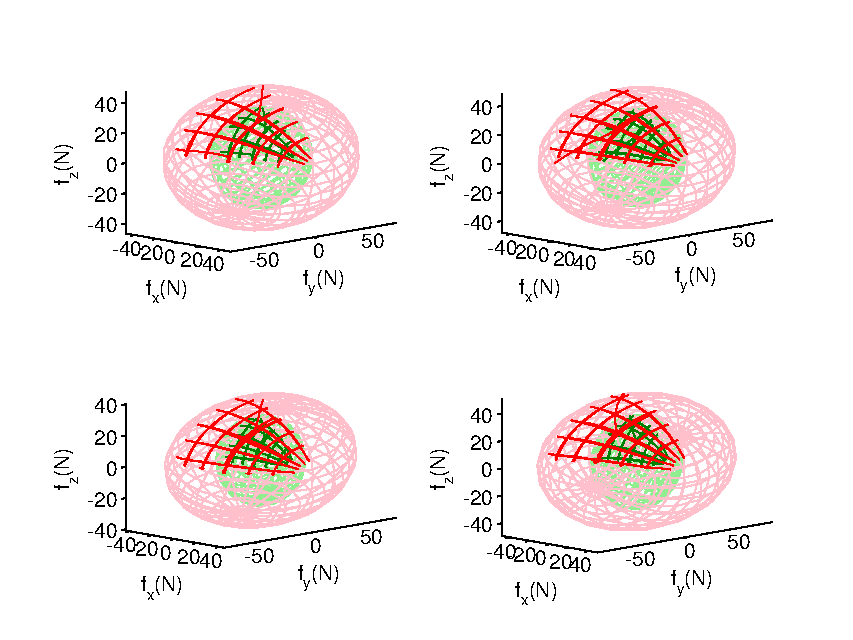
\includegraphics[width=0.65\textwidth]{images/leg_validation.pdf}}
\caption{The image shows the accuracy in calibrating the force/torque sensor
  with the procedure described in \cite{Traversaro2015b}. The four plots refer
  to four different experimental conditions (different values for the
  calibration weights).  Ideally, perfectly calibrated data should lie on the
  surface of a three dimensional sphere. Dark green: force measurements
  obtained with the calibration matrix estimated using the proposed
  technique. Dark red: force measurements obtained with the calibration matrix
  provided with the sensor.  Light red and light green surfaces: ellipsoids
  fitted to the measured forces.  Qualitative calibration accuracy can be
  obtained by looking at the spherical symmetry of the fitted ellipsoids.}
\label{fig:validation}
\end{figure}

 \begin{figure}
 \centering
 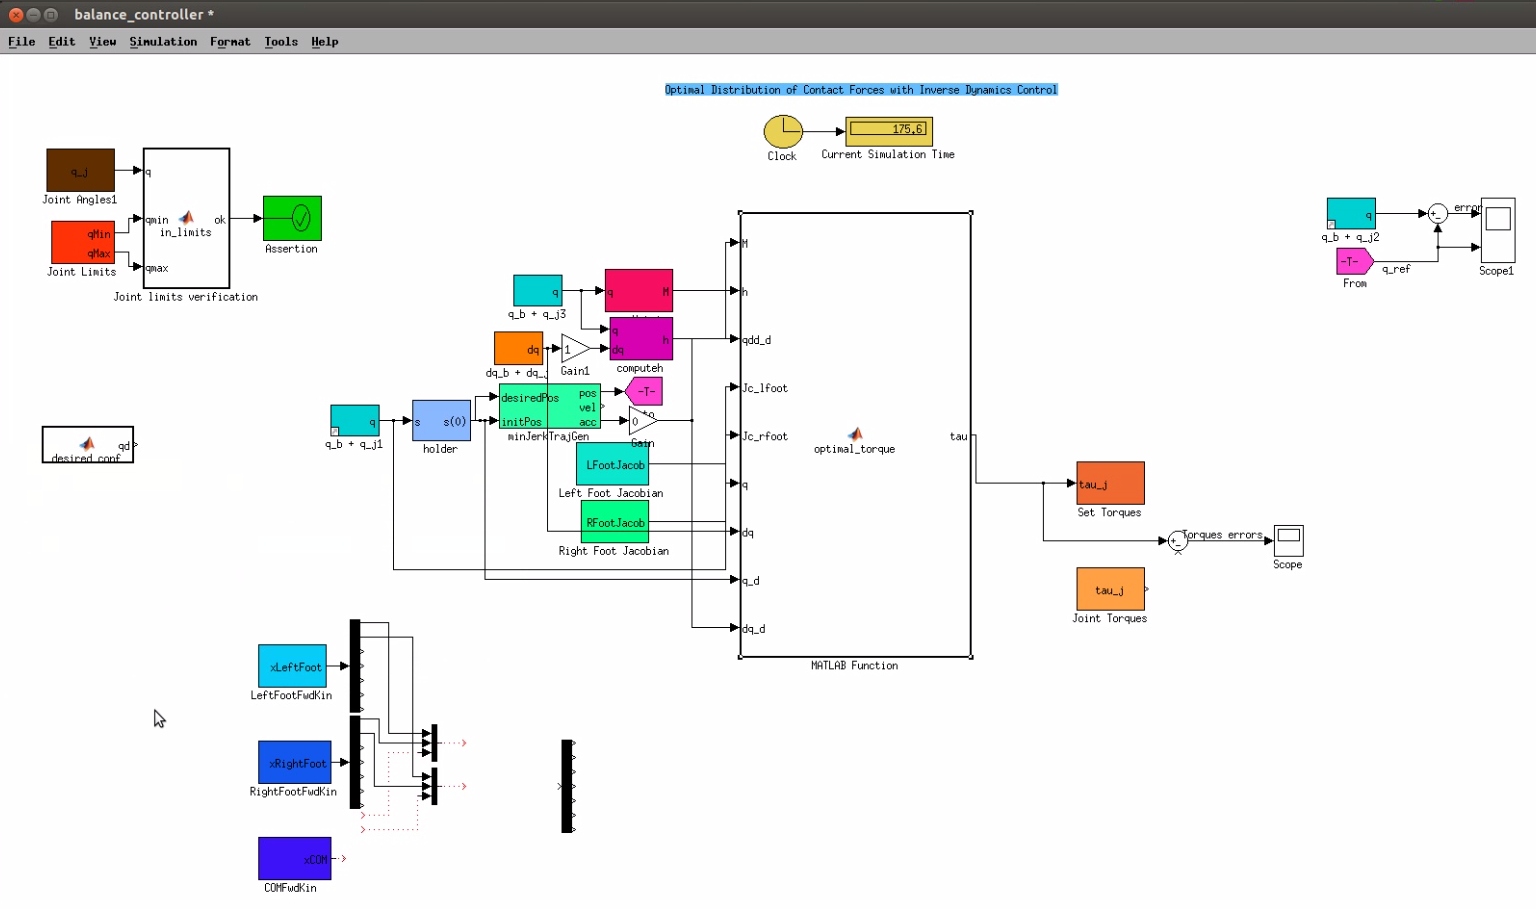
\includegraphics[width=0.7\textwidth]{wbi_torque_controller.png}
  \caption{One of the balance controllers implemented by TUD with the WBI
    toolbox in Matlab.  }
 \label{fig:wbitud}
 \end{figure}


\subparagraph{Extension and enhancement of the iDyn library. (T1.5)}
\label{sec:T15}
 
The goal of this task is to provide a reliable software tool for on-line
estimation of whole-body dynamics.  Before CoDyCo, dynamic estimations on the
iCub were relying on the iDyn software
library\footnote{\url{https://github.com/robotology/icub-main/tree/master/src/libraries/iDyn}.},
designed for fixed-base robots.  Within the first year of CoDyCo,
iDynTree\footnote{{\url{https://github.com/robotology/codyco/tree/master/src/libraries/iDynTree}}.}
was released in response to the need of representing floating base structures.
During the second year of the project, we investigated on the problem of
extending iDynTree to the case of multiple redundant sensors.  The
investigation resulted in an experimental software
library\footnote{\url{https://github.com/iron76/bnt_time_varying}.} currently
implemented in \textsc{Matlab}.  The software performs maximum-a-posteriori
dynamic estimation fusing multiple sensors such as gyroscopes, linear
accelerometers, embedded force-torque sensors and encoders.  Computational
efficiency is obtained by exploiting the sparsity of the underlying problem
\cite{Nori2015} (see Fig.~\ref{fig:varTimeComplete}).  Estimation accuracy is
obtained by a modified version of the expectation maximisation algorithm
\cite{Nori2015b} (see Fig.~\ref{fig:extForceEstimation}).

\begin{figure}
   \centering
   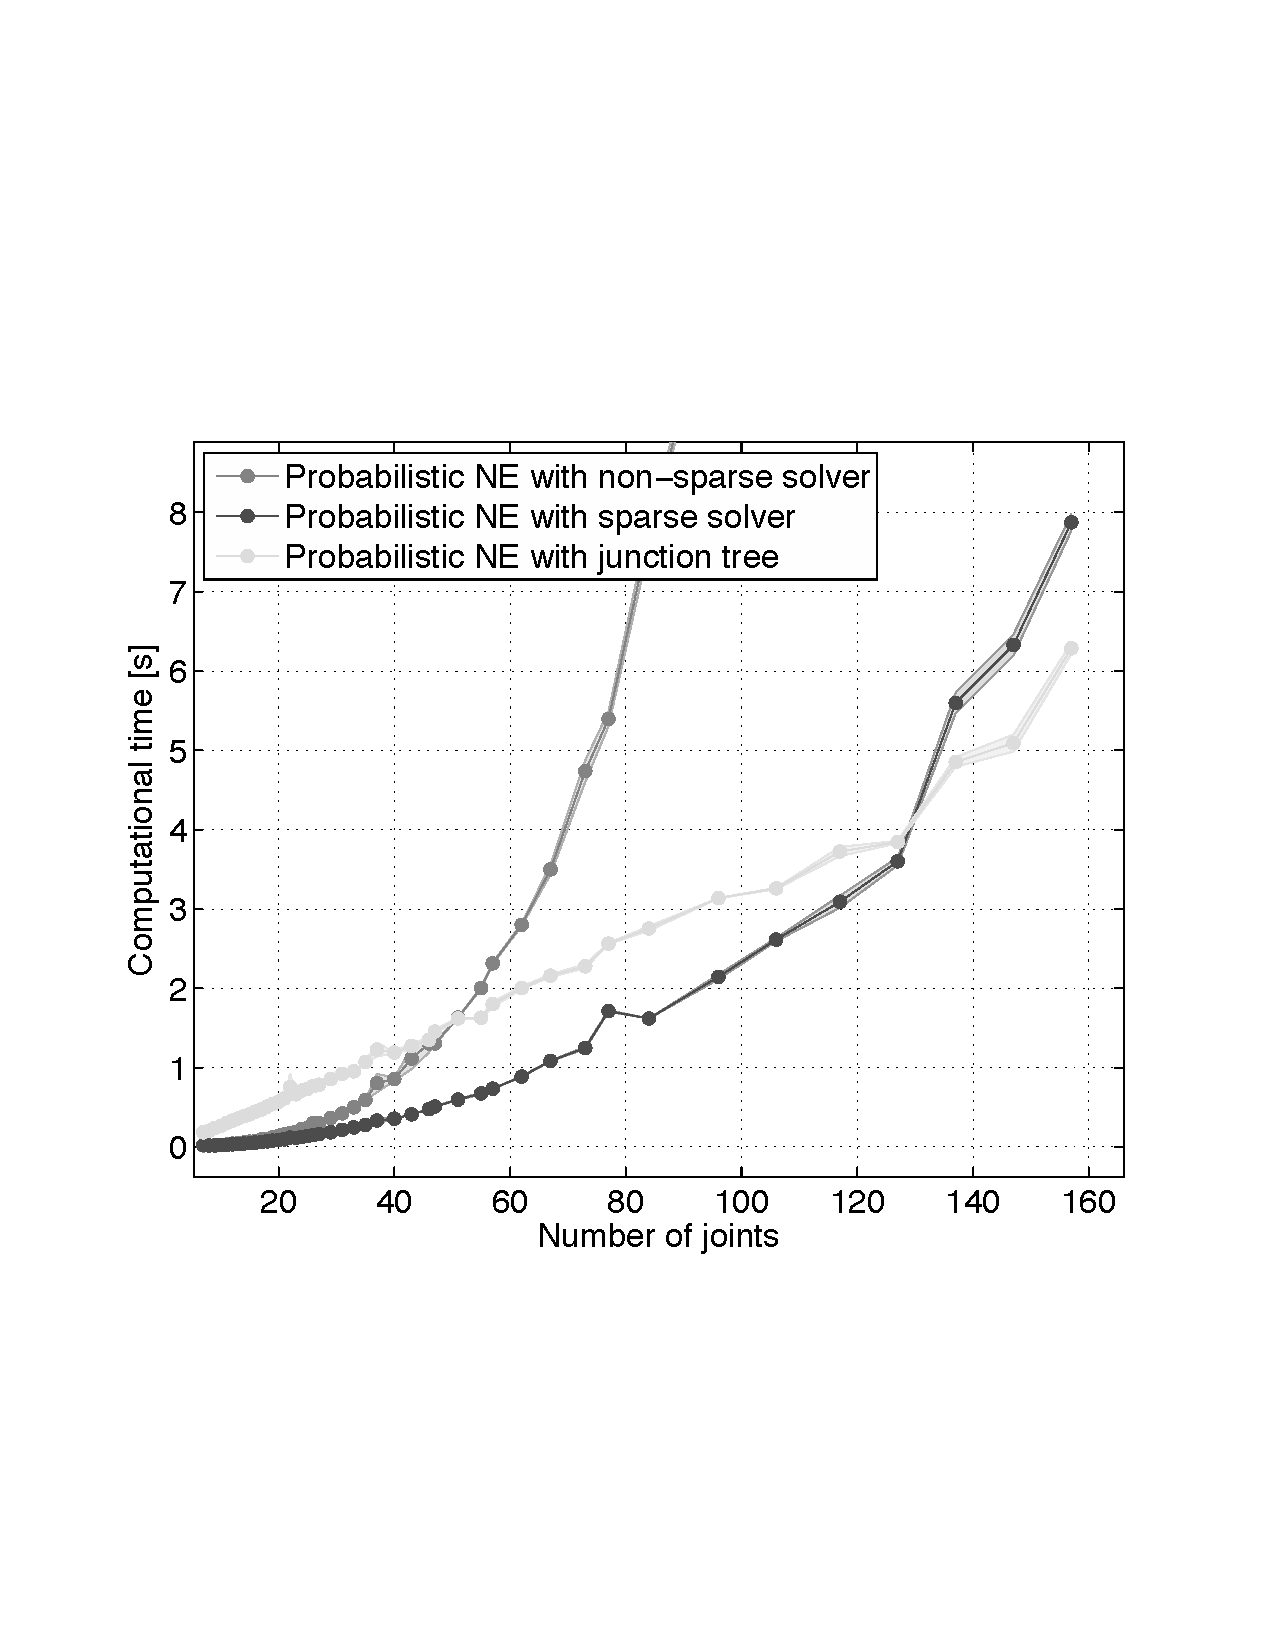
\includegraphics[height=0.35\hsize]{images/varTimeComplete.pdf}
   \caption{\label{fig:varTimeComplete} Comparison of non-sparse (S1-gray),
   sparse (S2-dark-gray) and Bayesian network junction tree (S3-light-gray)
   solvers in solving maximum-a-posteriori dynamics with redundant
   measurements (see \cite{Nori2015} for details).}
\end{figure}

\begin{figure*} [!ht]
  \centering
  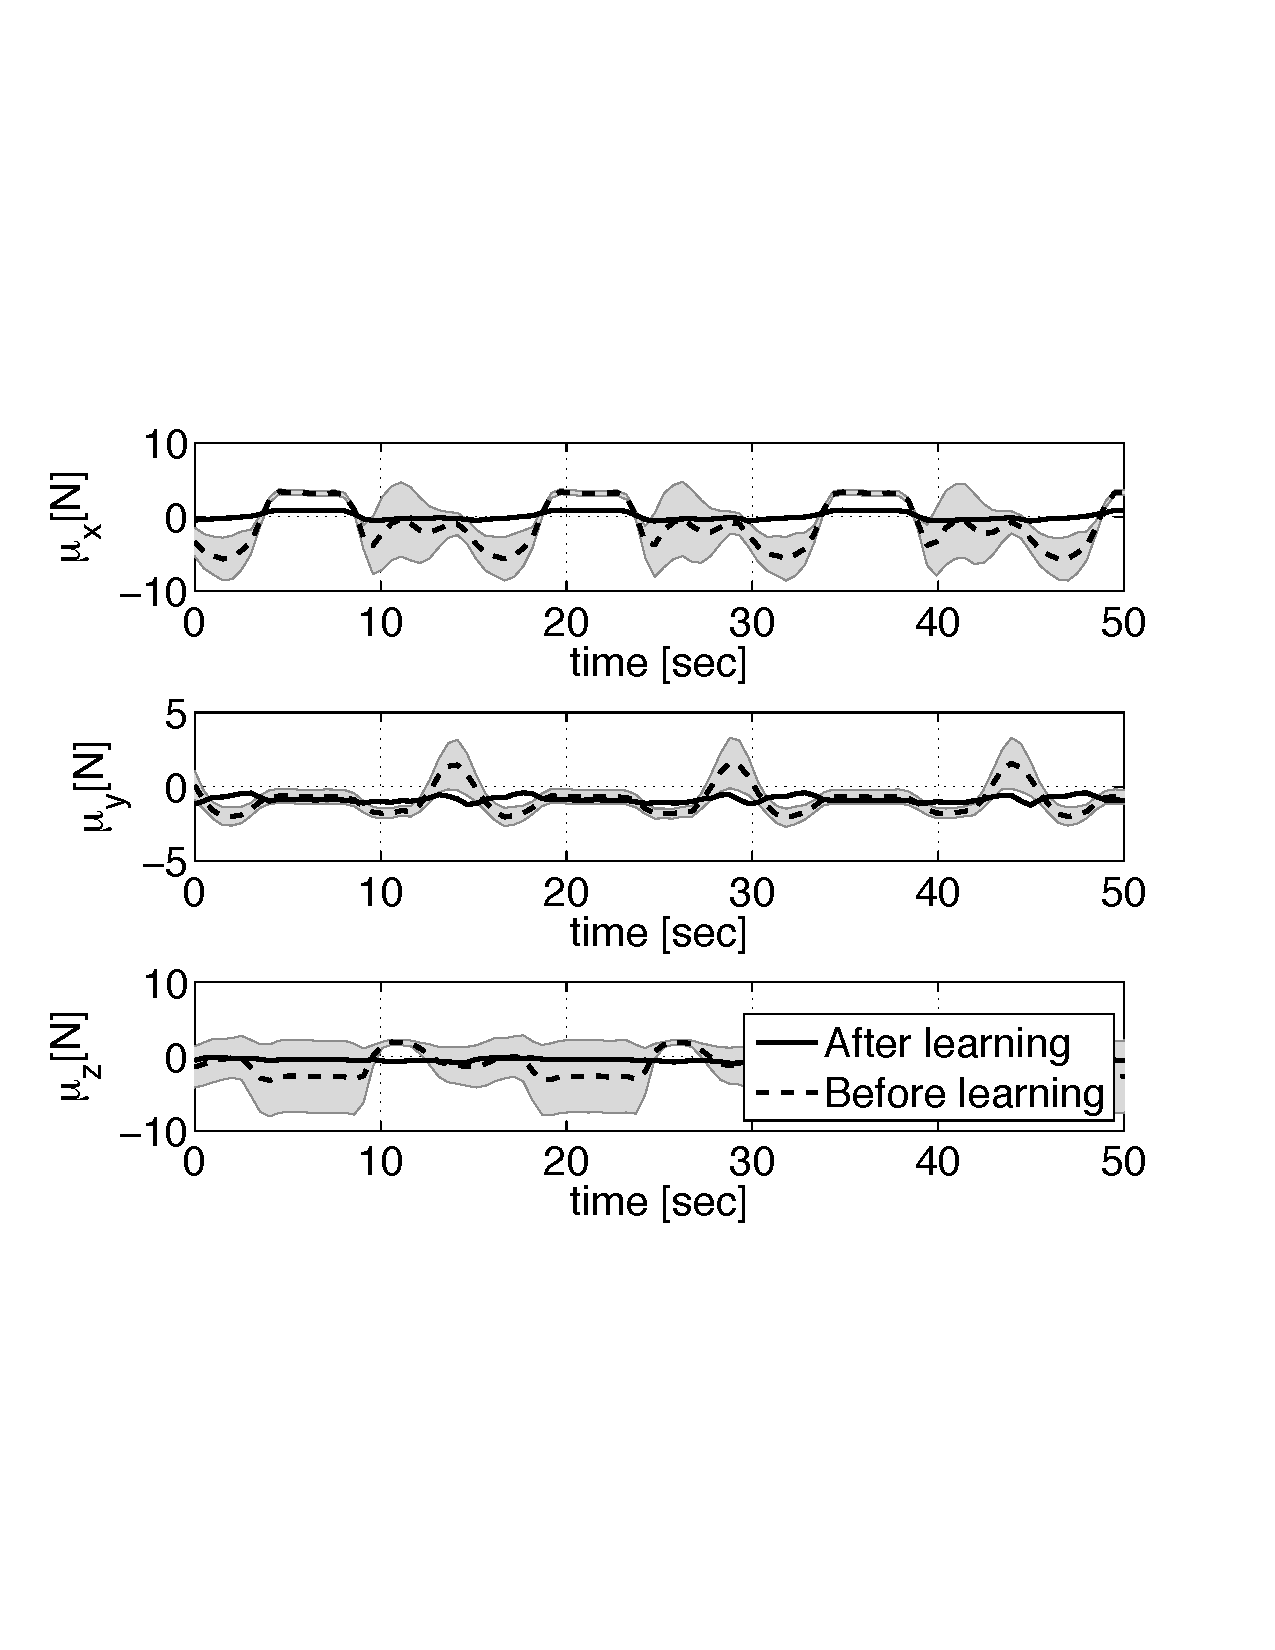
\includegraphics[width=0.45\hsize]{images/torques.pdf}
  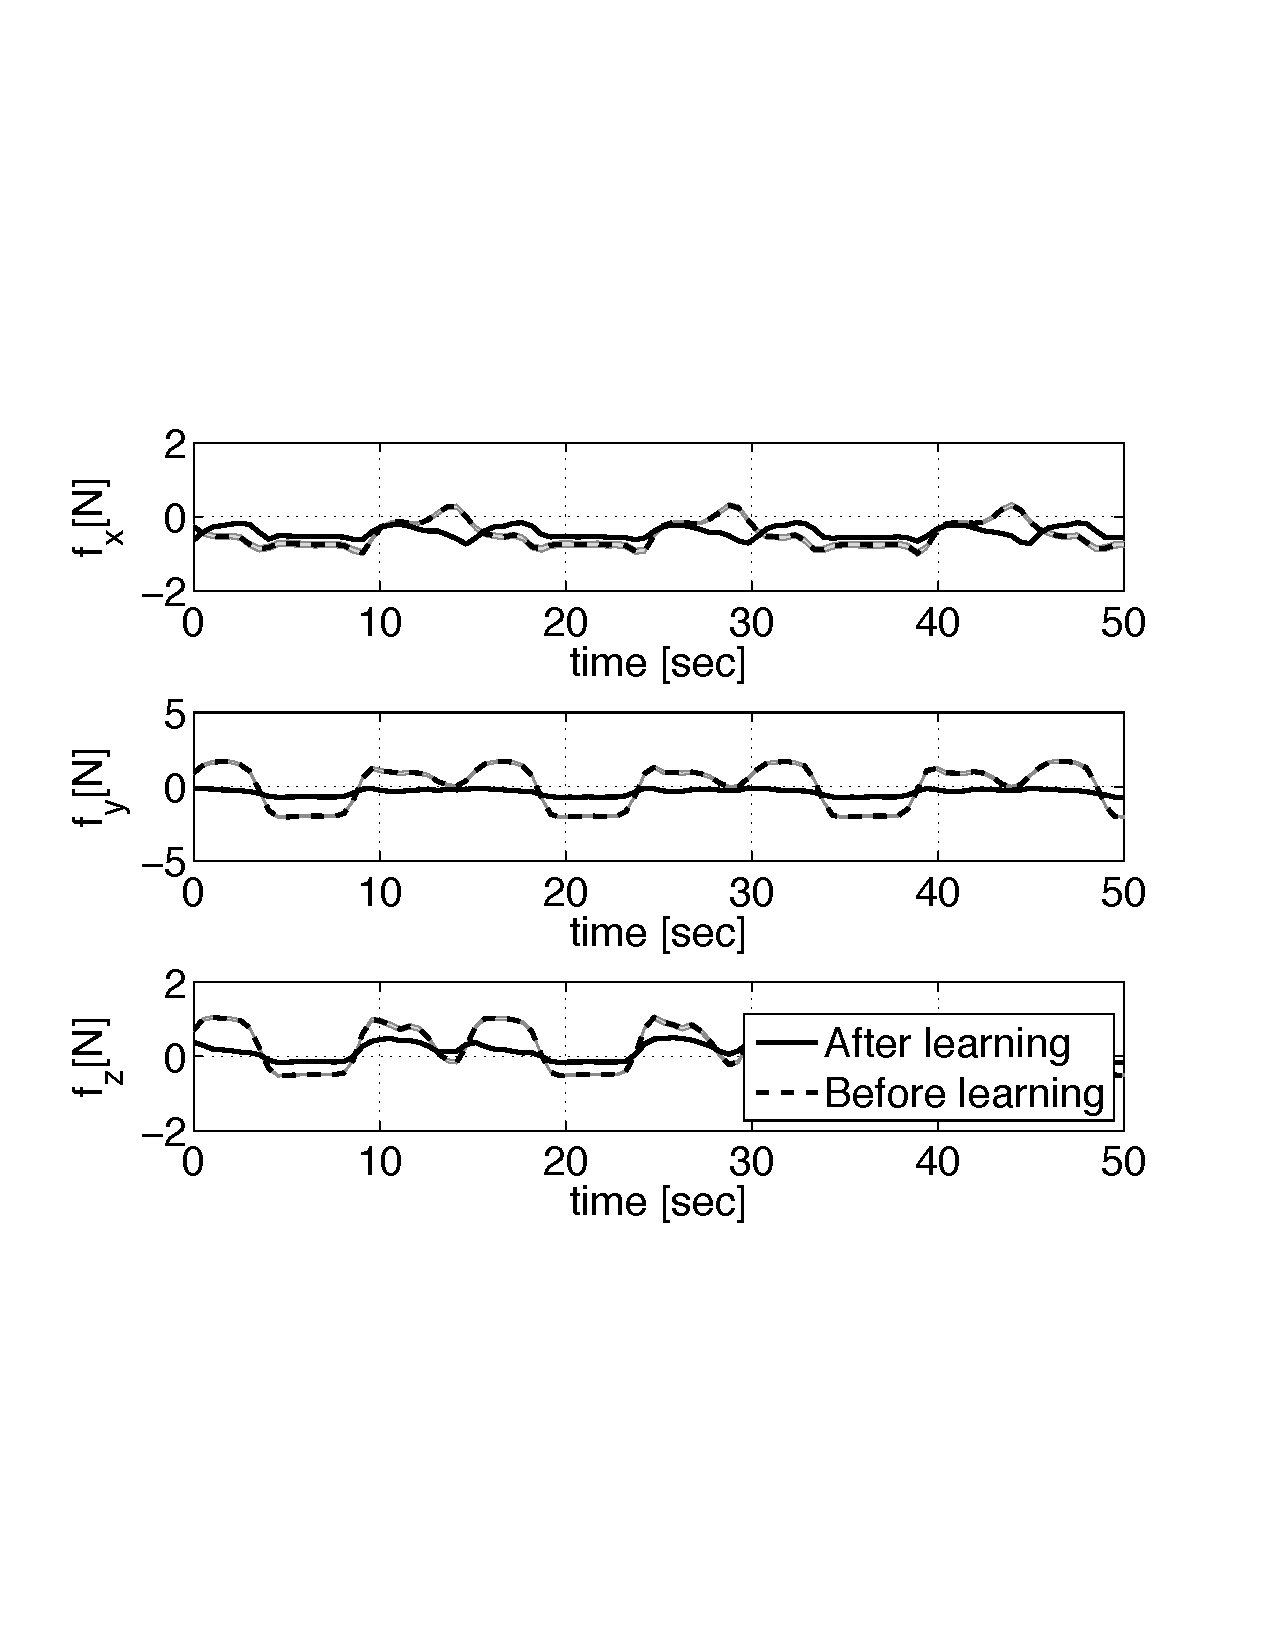
\includegraphics[width=0.45\hsize]{images/forces.pdf}
  \caption{\label{fig:extForceEstimation} The picture shows the errors in
  estimating an external wrench.  The two curves refer to the estimation
  obtained before (dashed line) and after (solid line) the estimation of the
  data covariance with a modified EM algorithm \cite{Nori2015b}.}
\end{figure*}











